\chapter{FUTURE OF MONEY}
\label{ch:Futureofmoney}

After the financial crisis of 2008, people learned the hard way that the financial markets did not only experienced so-called 'booms' but also suffered from the occasional 'busts'. Many people lost money one way or the other, and many more realized their high degree of exposure to a fraudulent system. Trust in the banks, governments and the financial sector took a huge hit and has not adequately recuperated since. 
Around the same time, in 2008, Satoshi Nakamoto released the Bitcoin whitepaper. \medskip

\tcbset{colback=orange!3!white,fonttitle=\bfseries}
    \begin{tcolorbox}
    [enhanced,
    title=Satoshi Nakamoto,
    frame style=
    {left color=orange!85!black,right color=yellow!95!black}]
    
       One of the fundamental properties of the Bitcoin protocol is that there will never be more than 21 million Bitcoins created, and there can never be more than 21 million Bitcoins in circulation. Economies and societies tend to do better when governed by a "fixed money supply" or a "sound money system". Economies tend to do poorly in an economy which is governed by the creation of unlimited amounts of fiat currency and an ever-increasing debt bubble. Therefore, the Bitcoin protocol is fundamentally different from the current (digital) fiat currency monetary system. On one end, there is Bitcoin with its fixed supply (sometimes referred to as the 'digital gold'). On the other end, there are the (digital) fiat currency economies that print currency into oblivion and create massive debt-based societies with asset price bubbles around the globe 
\end{tcolorbox}
\medskip 


\section{Gold or Bitcoin?}
Golds recent surge in price and longer-term bull market confirms that money transfers to what has always been a safe-haven asset in times of crisis (i.e. when fiat currencies fail or stock markets crash). This time around, besides traditional safe-haven assets, we have a digital equivalent - Bitcoin. Although it has not yet proven to be a real store of value over time like gold (because of extreme volatility and relatively low liquidity), younger generations might relate more to the "digital gold" of the 21st century than they relate with old-school physical gold. The first of its kind, Bitcoin originated (in essence) from the lack of trust as a result of the financial crisis in 2008 and will claim its fair market share as awareness of Bitcoin, blockchain and peer-to-peer cryptocurrencies grow.\medskip

\section*{Difference between Gold and Bitcoin}
The main difference between gold and Bitcoin is that Bitcoin is deflationary and gold is inflationary (average yearly gold supply growing with 2\%). If and when the system was to revert to a gold standard (or a "Bitcoin Standard" \parencite{bitcoinstandard}), it would drastically impact the monetary system. The financial and governmental institutions would have some restrictions and limitations in place. Thus the creation of financial products that add debt instead of long term value is restricted.


\section{The Blockchain [R]evolution}
Bitcoin utilises blockchain technology. While an important one, Bitcoin is only one use case for blockchain. Blockchain allows people to exchange assets and perform transactions without a third party. Imagine a world where you don't need intermediaries. While traditionally we have needed central authorities to trust one another and fulfil contracts, blockchain makes it possible to have our peers guarantee that for us. However, how?
Assets are no longer stored in a central place, but distributed across a global ledger, using the highest level of cryptography. When a participant conducts a transaction, it is broadcast to the network, which bundles, validates and records these transactions as blocks in a process called mining.

\medskip 
\tcbset{colback=orange!3!white,fonttitle=\bfseries}
    \begin{tcolorbox}
    [enhanced,
    title=Blockchain?,
    frame style=
    {left color=orange!85!black,right color=yellow!95!black}]
        
           \textit{The act of embedding a previous block of data into the current block of data is called chaining, hence, the name blockchain.}
       
\end{tcolorbox}
\medskip


\begin{figure}
    \centering
    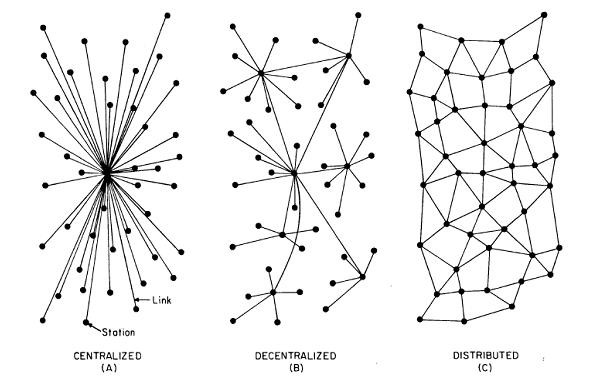
\includegraphics[width=.8\textwidth]{img/ch-exchanges/centralizedvsdecentralized.jpg}
    \caption[Centralized, decentralized and distributed architecture.]{Centralized, decentralized and distributed architecture. Bitcoin is a protocol and functions as a currency which runs on distributed ledger. \cite{lastamericanvagabond}}
    \label{fig:centralized_decentralized_distributed}

\end{figure}

\section{How Blockchain works}
Let us imagine a sheet of paper that has 25 lines. When the sheet is filled up with 25 transactions, the network validates the sheet (or block) via group consensus. Once the system approves the sheet, is added to a stack of previously approved sheets. Each sheet on the stack can be assumed to be trustworthy because, once a sheet is validated, it can't be changed. So to link our sheets together, we embed information from the previous sheet of paper into the new, recently validated sheet. In essence, a blockchain consists of bundled transactions in the form of blocks. \cite{course:blockchain_usecases}


To compromise or hack a blockchain network, someone would have to gain control of the majority of computers in that network. Hacking or otherwise tampering with a blockchain network is extremely difficult to do but not impossible. There is much debate about blockchain safety and security and potential bad actors using it with ill will. However, compared with traditional centralised infrastructures, there is no longer a single point of failure, and this is one of the main reasons why blockchain is infinitely more secure. Furthermore, multiple generations of blockchains already exist that work towards answering most of the other questions such as network liquidity, power consumptions, scalability and speed - all required to scale globally.\medskip 


\section{Huge potential but dangerous?}
In the long term even central banks or multilateral organizations' like the International Monetary Fund (IMF) will use this new technology - in the form of a central bank digital currency(CBDC) for instant payments. There are plenty of signs that indicate that distributed ledger technology might be used by some of these global agencies to implement their economic policies while making use of fiat cryptocurrencies (a digital product that they can inflate and control) \parencite{IMF_F&D}.


\begin{quotation}

      \textit{\say{In 1998 Wall Street bailed out the hedge funds. In 2008 central banks had to bail out Wall Street for them to survive. In the following crisis, whom do you think is going to bail out the central banks? }}
      \begin{flushright}
        \small{--- \textbf{J. Rickards}}
      \end{flushright}
    
\end{quotation}

\noindent Why do we address this in a cryptocurrency guide? Because we feel it's essential to look at both sides. This new technology has the potential to disrupt but can also be used to gain more control over populations (think 1984 by G. Orwell). For example, we are already heading towards a cashless society and less and less cash is accepted in the West. Think about factors such as e-cash, contact-less payments, credit cards, and mobile phone payments. Combine this with big data analysis of all the data we leave behind doing all sorts of social and economic transactions online. Think about your shadow identity that exists online, which is a trail of breadcrumbs left behind by you, during your time online. Google, Apple, Amazon and Facebook most likely know you better than yourself, in terms of what triggers you and what you did a few years ago on a particular day. Please take a look at China, for example, where they have implemented and are experimenting with social credit scores of individuals. China uses credit scores, obtained from cameras, online surveillance and big data analysis to rank citizens and provide either certain perks or take perks away, pending your score \parencite{chinasocialscores}. These practices drastically affect the lives of millions of individuals. You might be severely discriminated, depending on your ability to conform to this expected behaviour and if show compliance to the \say{model citizen}. Moreover, Western banks are already working with scoring cards to check if you're allowed to receive credit. So these processes are already present here, although much less extreme.\medskip


\begin{quotation}

      \textit{\say{Technology is a force multiplier, it can be used for good and bad purpose}}
      \begin{flushright}
        \small{--- \textbf{Cryptomanuals}}
      \end{flushright}
    
\end{quotation}

\section{Technology has no agenda, People do}
It is essential to realize that technology has no personal agenda or objective and can be used and utilized by its creators as seen fit. For example, planes and ships are used for both civilian and military purposes. Also, it would be safe to assume that the inventor of the wheel never anticipated Formula 1 race cars or sophisticated tanks. These are extreme examples but only serve to illustrate the fact that technology is just a tool which can be used for either good or bad things, depending on many factors.\medskip 

Distributed ledger technology originated (in essence) from the financial crisis in 2008 and is here to stay. The question remains how we are going to apply this technology to utilize it to its fullest potential. 


\section{Financial-Technology Sector}
Besides, this market has enormous potential when you think of the possibilities for potential growth on investments in the long term since it is still in its infancy stages. Some of these projects are here to stay, and many more are starting every day, introducing healthy competition that is going to boost the fin-tech industry. There is an ever-increasing demand for skilled people in the fin-tech sector. Businesses cannot seem to find enough software engineers and blockchain developers, and everyone can get into it - take several free courses available on the internet to get you up to speed and develop new skill-sets that might boost your career and give you a new direction - this industry is just getting started. Not to mention the fact that the younger generations have been growing up in the digital age and the impact this makes on their lives cannot be unseen.\medskip

Mainly, the success of blockchain technology has already been set in stone since it's not dependent on cryptocurrency alone. Where blockchain can serve as a decentralised ledger that securely stores immutable data, we can also use it as such without the use of any cryptocurrencies. Cryptocurrencies or tokens might be used on specific networks because they have a serve a particular function. They might function as a utility token or as a means of payment to the network or to store, capture or move value around in the form of a digital currency.\medskip


\section{Blockchain is Here to Stay}
We believe blockchain is here to stay, and it will be an integral element in our future infrastructure. The challenge is to oversee and guide the adoption process. For example, it is almost inevitable that private blockchain infrastructures are going to be used by governments and corporations. Good or bad? That's a loaded question as there might be more than one answer. Even though it may sound bad for cryptocurrency or blockchain in general - adaptive governments and nimble and experimental regulation, legislation and compliance policies will be of crucial importance to propel development forward. 

Besides Bitcoin, there are hundreds of other projects out there that are working on solving some of the most pressing matters in our financial spheres and other industries like supply chain, healthcare, energy and content creation. We believe blockchain is here to stay, and it will be an integral element in our future infrastructure.  The challenge is to oversee and guide the adoption process.

\section{Open Blockchain Enables Inclusion}
Cryptocurrencies, particularly Bitcoin, already have massive momentum. We are not predicting whether or not all of this will eventually succeed. However, we do believe that the economy works best when it works for everyone, and this new platform represents an engine which stimulates and enables inclusion. Open blockchain significantly lowers the requirements for people to obtain access to financial services and will compete with traditional central banking models. With Bitcoin, it is also completely different in terms of spending. Open blockchains like Bitcoins do not care; they are peer to peer. You can send it from person to person, without an intermediary. 

In summary, when you store money at the bank (or in the possible future at corporations), the bank becomes the owner of that money. With Bitcoin, \emph{you} own your money. When the banks own that money, they spend it as they wish. When you own it, \emph{you} spend it as you wish. It is censorship-resistant, and no one decides on what you can or cannot spend it.\medskip 

